\part{Présentation des sources primaires}
\chapter{}
\section{Presentation}
Pour répondre à cette problématique, j’ai à ma disposition trois types de sources primaires:
\begin{itemize}
 \item{Les données de la base des « Militaires décédés sur les théâtres d'opérations extérieurs (1905-1962) ».\footnote{\url{https://www.memoiredeshommes.sga.defense.gouv.fr/fr/article.php?larub=46&titre=militaires-decedes-sur-les-theatres-d-operations-exterieurs-1905-1962-}}}
\item{Les registres matricules, qui sont numérisés sur le site \underline{Mémoire des hommes} mais seulement jusqu'à 1918.\footnote{\url{https://www.memoiredeshommes.sga.defense.gouv.fr/fr/article.php?larub=382&titre=recensement-des-engages-et-appeles-des-anciennes-colonies-francaises}}}
\item{Les journaux des marches et opérations des régiments ayant participé à la guerre du Rif, qui ne sont pas numérisés.\footnote{Dans les fonds du SHD sur la Maroc (serie 3H).}}
\end{itemize}
Il existe sûrement d’autres documents d’archives qui traitent de la pluralité des soldats ayant participé à la guerre du Rif dans les archives des officiers supérieurs, généraux, administrateurs et personnalités qui ont contribué à la conduite de la guerre et à l’administration du protectorat du Maroc. Au niveau individuel et à grande échelle, je ne dispose que ses trois objets historiques.\\ 
\section{La base de données de morts}
Cette base de données devrait contenir tous les morts de l’armée française en dehors du sol national pendant la période spécifiée (1905-1962). Ces dates correspondent au début des affrontements entre le Maroc et la France et à la fin de la guerre de l’Algérie. Après cette période, lors de la création de la Vème République, le concept d'opération extérieure a été  créé pour désigner les conflits et opérations des armées françaises en dehors de la métropole. Avant la création du concept, les forces armées françaises ont entrepris des opérations très  variées sans nom particulier . Elles pouvaient se dérouler  en territoire ennemi comme l’Allemagne, ou encore en Russie pendant la guerre civile ou au Maroc ou alors sur un autre territoire de l’empire français. Ce que j’essaie de souligner, est que la terminologie «opérations extérieures » de cette base de données ne correspond à aucune nomenclature militaire ou politique. Ce manque d'homogénéité dans la nature  des opérations menées incluses dans cette base est visible dans sa composition diplomatique. Les informations contenues dans la base proviennent de plusieurs types de documents tels que des fiches individuelles de décès ou des statuts de pension militaire. Pour être encore plus précis, elles proviennent de deux archives spécifiques du SHD : la Division des Archives des Victimes des Conflits Contemporains (DAVCC) du Service historique de la défense à Caen et les archives de la sous-direction des pensions militaires à la Rochelle. À partir de la réunion des fonds des côtes 40 R, 35 R et 36 R pour les fiches individuelles de décès en provenance de la DAVCC et de fonds inconnus des pensions militaires de la Rochelle, une équipe sous la direction de Christophe Dupont a procédé à la transcription et l’encodage de la base de données en question qui a été publiée en 2012. Depuis sa mise en ligne, la base a continué à évoluer avec des mises à jour périodiques de nouvelles données. Grâce à un travail de volontariat des internautes, les informations manquantes ont pu être complétées avec des fiches de matricules. Du coup la base n’est plus évolutive aujourd’hui. \footnote{Information provenant d’un entretien téléphonique avec la  Division des Archives des Victimes des Conflits Contemporains du SHD, de Caen, un échange par mail avec M. Christophe Dupont (24/05/2022) et du site \href{https://www.memoiredeshommes.sga.defense.gouv.fr/fr/article.php?laref=69&titre=aide-a-la-recherche}{\underline{Mémoire des hommes}}. }\\

Comme pour l'ensemble du site Mémoire des hommes, le SHD utilise le logiciel de gestion de site web et données d’archives publiques proposé par l’entreprise \href{http://www.arkotheque.fr/}{\underline{Arkothèque}}. Cette interface permet de télécharger et de naviguer dans la base de données selon plusieurs critères : ceux de l’état civil du soldat décédé, et si le cas le permet, des détails plus précis comme le conflit où il a combattu,et les détails de sa mort ou son grade. Elle permet aussi de différencier les titres que la hiérarchie militaire a attribués à la mort de chacun des ces soldats, par exemple: « mort pour la France », non-statué ou inconnu. Ces recherches sont effectuées avec le moteur d’Arkothèque qui fonctionne sur la  base de \textbf{javascript}.\footnote{Voir annexe : \ref{fig:Arkothèque 1}, \ref{fig:Arkothèque 2}.} Cela limite les possibilités de faire un scrapping ciblé de la base de données. Heureusement, la base de données peut être téléchargée sous format CSV. La figure 1 représente un échantillon réduit du tableau brut de la base de données.\begin{figure}[H]
    \hspace*{-2cm} 
    \caption{La base de données en format CSV}
    \label{fig:1}
     \begin{adjustwidth}{-2cm}{}
\begin{longtable}[c]{llllllllllllllllllllllllllllllllllllllllllllllllllllllllllllllllllllllllll}
id\_conflit\_intitule & id\_sous\_conflit\_intitule & id\_famille\_cote\_intitule & sous\_serie & serie & article & nom & prenom & nom\_autre & pseudonyme & naissance\_jour\_mois\_annee & id\_naissance\_lieu\_intitule & id\_naissance\_departement\_intitule & id\_naissance\_pays\_intitule & id\_statut\_intitule & id\_mention\_intitule & classe & recrutement\_matricule & id\_recrutement\_bureau\_intitule & id\_grade\_intitule & id\_unite\_intitule & id\_bataillon\_intitule & id\_compagnie\_intitule & id\_batterie\_intitule & detail\_unite & id\_profession\_intitule & deces\_jour\_mois\_annee & id\_deces\_lieu\_intitule & id\_deces\_departement\_intitule & id\_deces\_pays\_intitule & id\_operation\_intitule & id\_transcription\_etablissement\_lieu\_intitule & id\_transcription\_etablissement\_departement\_intitule & id\_transcription\_etablissement\_pays\_intitule & id\_dernier\_domicile\_lieu\_intitule & id\_dernier\_domicile\_departement\_intitule & id\_dernier\_domicile\_pays\_intitule & id\_sepulture\_lieu\_intitule & id\_sepulture\_departement\_intitule & id\_sepulture\_pays\_intitule & id\_sepulture\_nom\_du\_site\_intitule & id\_sepulture\_type\_intitule & sepulture\_carre & sepulture\_rang & sepulture\_tombe\_individuelle\_numero & sepulture\_tombe\_indice & id\_sepulture\_lieu\_premiere\_inhumation\_intitule & id\_lieu\_incarceration\_intitule & sources & cote & id\_region\_militaire\_intitule & deportation & id\_decoration\_intitule & decoration\_posthume & decret & jo & id\_mdh\_base\_nominative\_lien\_famille\_resistance\_les\_intitules & id\_mdh\_base\_nominative\_lien\_nom\_mouvement\_rif\_les\_intitules & id\_mdh\_base\_nominative\_lien\_nom\_reseau\_ffc\_les\_intitules & rehabilitation & rehabilitation\_detail & site\_conservation & lien\_ark\_fiche & corps\_retrouve & disparition\_date\_libre & disparition\_jour\_mois\_annee & jdd\_jour\_mois\_annee & disparition\_lieu\_complement & id\_disparition\_lieu\_intitule & id\_disparition\_departement\_intitule & id\_disparition\_pays\_intitule & id\_tgi\_lieu\_intitule & id\_tgi\_departement\_intitule & id\_tgi\_pays\_intitule \\
\endfirsthead
%
\endhead
%
Théâtres d'opérations extérieurs & Afrique du Nord &  &  &  &  & AB EL OUAHAB BEN SAID BEN BELGACEM &  &  &  & 0000-00-00 &  &  &  &  & Non Mort pour la France &  &  &  & soldat & 20e régiment de tirailleurs (20e RT) &  &  &  &  &  & 08/10/1925 & Taza &  & Maroc &  &  &  &  &  &  &  &  &  &  &  &  &  &  &  &  &  &  & Service historique de la Défense, Caen &  &  & 0 &  & 0 &  &  &  &  &  & 0 &  &  & https://www.memoiredeshommes.sga.defense.gouv.fr/fr/ark:/40699/m00523bec44c8132 & 0 &  &  &  &  &  &  &  &  &  &  \\
Théâtres d'opérations extérieurs & Levant & AC & 40 & R & 4063 & ABABOA &  &  &  &  &  &  &  &  & Non Mort pour la France &  &  &  & soldat &  &  &  &  &  &  & 19/07/1920 & Tarsous &  & Cilicie &  & Lavigerie &  & Algérie &  &  &  &  &  &  &  &  &  &  &  &  &  &  & Service historique de la Défense, Caen &  &  & 0 &  & 0 &  &  &  &  &  & 0 &  &  & https://www.memoiredeshommes.sga.defense.gouv.fr/fr/ark:/40699/m00523be53d49952 & 0 &  &  &  &  &  &  &  &  &  &  \\
Théâtres d'opérations extérieurs & Levant & AC & 40 & R & 4063 & ABABOU & Abdelkader &  &  &  &  &  &  &  & Non Mort pour la France &  &  &  & sergent & 18e régiment de tirailleurs (18e RT) &  &  &  &  &  & 11/04/1920 & Ourfa &  & Cilicie &  & Les Attafs &  & Algérie &  &  &  &  &  &  &  &  &  &  &  &  &  &  & Service historique de la Défense, Caen &  &  & 0 &  & 0 &  &  &  &  &  & 0 &  &  & https://www.memoiredeshommes.sga.defense.gouv.fr/fr/ark:/40699/m00523be2909f48a & 0 &  &  &  &  &  &  &  &  &  &  \\
Théâtres d'opérations extérieurs & Afrique du Nord & AC & 40 & R & 4034 & ABABSA & Belgacem &  &  &  &  &  &  &  & Non Mort pour la France &  &  &  & soldat & 11e régiment de tirailleurs (11e RT) &  &  &  &  &  & 16/08/1923 & Ahl Telt &  & Maroc &  & Khenchela (ex département de Constantine) &  & Algérie &  &  &  &  &  &  &  &  &  &  &  &  &  &  & Service historique de la Défense, Caen &  &  & 0 &  & 0 &  &  &  &  &  & 0 &  &  & https://www.memoiredeshommes.sga.defense.gouv.fr/fr/ark:/40699/m00523be18c4cba3 & 0 &  &  &  &  &  &  &  &  &  & 
\end{longtable}
\begin{longtable}[c]{llllllllllllllllllllllllllllllllllllllllllllllllllllllllllllllllllllll}
serie & article & nom & prenom & nom\_autre & pseudonyme & naissance\_jour\_mois\_annee & id\_naissance\_lieu\_intitule & id\_naissance\_departement\_intitule & id\_naissance\_pays\_intitule & id\_statut\_intitule & id\_mention\_intitule & classe & recrutement\_matricule & id\_recrutement\_bureau\_intitule & id\_grade\_intitule & id\_unite\_intitule & id\_bataillon\_intitule & id\_compagnie\_intitule & id\_batterie\_intitule & detail\_unite & id\_profession\_intitule & deces\_jour\_mois\_annee & id\_deces\_lieu\_intitule & id\_deces\_departement\_intitule & id\_deces\_pays\_intitule & id\_operation\_intitule & id\_transcription\_etablissement\_lieu\_intitule & id\_transcription\_etablissement\_departement\_intitule & id\_transcription\_etablissement\_pays\_intitule & id\_dernier\_domicile\_lieu\_intitule & id\_dernier\_domicile\_departement\_intitule & id\_dernier\_domicile\_pays\_intitule & id\_sepulture\_lieu\_intitule & id\_sepulture\_departement\_intitule & id\_sepulture\_pays\_intitule & id\_sepulture\_nom\_du\_site\_intitule & id\_sepulture\_type\_intitule & sepulture\_carre & sepulture\_rang & sepulture\_tombe\_individuelle\_numero & sepulture\_tombe\_indice & id\_sepulture\_lieu\_premiere\_inhumation\_intitule & id\_lieu\_incarceration\_intitule & sources & cote & id\_region\_militaire\_intitule & deportation & id\_decoration\_intitule & decoration\_posthume & decret & jo & id\_mdh\_base\_nominative\_lien\_famille\_resistance\_les\_intitules & id\_mdh\_base\_nominative\_lien\_nom\_mouvement\_rif\_les\_intitules & id\_mdh\_base\_nominative\_lien\_nom\_reseau\_ffc\_les\_intitules & rehabilitation & rehabilitation\_detail & site\_conservation & lien\_ark\_fiche & corps\_retrouve & disparition\_date\_libre & disparition\_jour\_mois\_annee & jdd\_jour\_mois\_annee & disparition\_lieu\_complement & id\_disparition\_lieu\_intitule & id\_disparition\_departement\_intitule & id\_disparition\_pays\_intitule & id\_tgi\_lieu\_intitule & id\_tgi\_departement\_intitule & id\_tgi\_pays\_intitule \\
\endfirsthead
%
\endhead
%
 &  & AB EL OUAHAB BEN SAID BEN BELGACEM &  &  &  & 0000-00-00 &  &  &  &  & Non Mort pour la France &  &  &  & soldat & 20e régiment de tirailleurs (20e RT) &  &  &  &  &  & 08/10/1925 & Taza &  & Maroc &  &  &  &  &  &  &  &  &  &  &  &  &  &  &  &  &  &  & Service historique de la Défense, Caen &  &  & 0 &  & 0 &  &  &  &  &  & 0 &  &  & https://www.memoiredeshommes.sga.defense.gouv.fr/fr/ark:/40699/m00523bec44c8132 & 0 &  &  &  &  &  &  &  &  &  &  \\
R & 4063 & ABABOA &  &  &  &  &  &  &  &  & Non Mort pour la France &  &  &  & soldat &  &  &  &  &  &  & 19/07/1920 & Tarsous &  & Cilicie &  & Lavigerie &  & Algérie &  &  &  &  &  &  &  &  &  &  &  &  &  &  & Service historique de la Défense, Caen &  &  & 0 &  & 0 &  &  &  &  &  & 0 &  &  & https://www.memoiredeshommes.sga.defense.gouv.fr/fr/ark:/40699/m00523be53d49952 & 0 &  &  &  &  &  &  &  &  &  &  \\
R & 4063 & ABABOU & Abdelkader &  &  &  &  &  &  &  & Non Mort pour la France &  &  &  & sergent & 18e régiment de tirailleurs (18e RT) &  &  &  &  &  & 11/04/1920 & Ourfa &  & Cilicie &  & Les Attafs &  & Algérie &  &  &  &  &  &  &  &  &  &  &  &  &  &  & Service historique de la Défense, Caen &  &  & 0 &  & 0 &  &  &  &  &  & 0 &  &  & https://www.memoiredeshommes.sga.defense.gouv.fr/fr/ark:/40699/m00523be2909f48a & 0 &  &  &  &  &  &  &  &  &  &  \\
R & 4034 & ABABSA & Belgacem &  &  &  &  &  &  &  & Non Mort pour la France &  &  &  & soldat & 11e régiment de tirailleurs (11e RT) &  &  &  &  &  & 16/08/1923 & Ahl Telt &  & Maroc &  & Khenchela (ex département de Constantine) &  & Algérie &  &  &  &  &  &  &  &  &  &  &  &  &  &  & Service historique de la Défense, Caen &  &  & 0 &  & 0 &  &  &  &  &  & 0 &  &  & https://www.memoiredeshommes.sga.defense.gouv.fr/fr/ark:/40699/m00523be18c4cba3 & 0 &  &  &  &  &  &  &  &  &  & 
\end{longtable}
\begin{longtable}[c]{llllllllllllllllllllllllllllllllllllllllllllllllll}
id\_mention\_intitule & id\_grade\_intitule & id\_unite\_intitule & deces\_jour\_mois\_annee & id\_deces\_lieu\_intitule & id\_deces\_pays\_intitule & id\_operation\_intitule & id\_transcription\_etablissement\_lieu\_intitule & id\_transcription\_etablissement\_departement\_intitule & id\_transcription\_etablissement\_pays\_intitule & id\_dernier\_domicile\_lieu\_intitule & id\_dernier\_domicile\_departement\_intitule & id\_dernier\_domicile\_pays\_intitule & id\_sepulture\_lieu\_intitule & id\_sepulture\_departement\_intitule & id\_sepulture\_pays\_intitule & id\_sepulture\_nom\_du\_site\_intitule & id\_sepulture\_type\_intitule & sepulture\_carre & sepulture\_rang & sepulture\_tombe\_individuelle\_numero & sepulture\_tombe\_indice & id\_sepulture\_lieu\_premiere\_inhumation\_intitule & id\_lieu\_incarceration\_intitule & sources & cote & id\_region\_militaire\_intitule & deportation & id\_decoration\_intitule & decoration\_posthume & decret & jo & id\_mdh\_base\_nominative\_lien\_famille\_resistance\_les\_intitules & id\_mdh\_base\_nominative\_lien\_nom\_mouvement\_rif\_les\_intitules & id\_mdh\_base\_nominative\_lien\_nom\_reseau\_ffc\_les\_intitules & rehabilitation & rehabilitation\_detail & site\_conservation & lien\_ark\_fiche & corps\_retrouve & disparition\_date\_libre & disparition\_jour\_mois\_annee & jdd\_jour\_mois\_annee & disparition\_lieu\_complement & id\_disparition\_lieu\_intitule & id\_disparition\_departement\_intitule & id\_disparition\_pays\_intitule & id\_tgi\_lieu\_intitule & id\_tgi\_departement\_intitule & id\_tgi\_pays\_intitule \\
\endfirsthead
%
\endhead
%
Non Mort pour la France & soldat & 20e régiment de tirailleurs (20e RT) & 08/10/1925 & Taza & Maroc &  &  &  &  &  &  &  &  &  &  &  &  &  &  &  &  &  &  & Service historique de la Défense, Caen &  &  & 0 &  & 0 &  &  &  &  &  & 0 &  &  & https://www.memoiredeshommes.sga.defense.gouv.fr/fr/ark:/40699/m00523bec44c8132 & 0 &  &  &  &  &  &  &  &  &  &  \\
Non Mort pour la France & soldat &  & 19/07/1920 & Tarsous & Cilicie &  & Lavigerie &  & Algérie &  &  &  &  &  &  &  &  &  &  &  &  &  &  & Service historique de la Défense, Caen &  &  & 0 &  & 0 &  &  &  &  &  & 0 &  &  & https://www.memoiredeshommes.sga.defense.gouv.fr/fr/ark:/40699/m00523be53d49952 & 0 &  &  &  &  &  &  &  &  &  &  \\
Non Mort pour la France & sergent & 18e régiment de tirailleurs (18e RT) & 11/04/1920 & Ourfa & Cilicie &  & Les Attafs &  & Algérie &  &  &  &  &  &  &  &  &  &  &  &  &  &  & Service historique de la Défense, Caen &  &  & 0 &  & 0 &  &  &  &  &  & 0 &  &  & https://www.memoiredeshommes.sga.defense.gouv.fr/fr/ark:/40699/m00523be2909f48a & 0 &  &  &  &  &  &  &  &  &  &  \\
Non Mort pour la France & soldat & 11e régiment de tirailleurs (11e RT) & 16/08/1923 & Ahl Telt & Maroc &  & Khenchela (ex département de Constantine) &  & Algérie &  &  &  &  &  &  &  &  &  &  &  &  &  &  & Service historique de la Défense, Caen &  &  & 0 &  & 0 &  &  &  &  &  & 0 &  &  & https://www.memoiredeshommes.sga.defense.gouv.fr/fr/ark:/40699/m00523be18c4cba3 & 0 &  &  &  &  &  &  &  &  &  & 
\end{longtable}
\end{adjustwidth}
\end{figure}Le tableau comporte plusieurs colonnes qui indiquent les caractéristiques de chaque soldat. C’est à partir des informations contenues dans ces colonnes que notre analyse peut débuter. La répartition des données n’est pas égale entre tous les soldats. On peut trouver des cas très détaillés et d’autres avec juste une date et un pays de décès. La base brute comprend 20.059 individus morts de 1905-1962.
\section{Les registres matricules}
Les registres matricules sont les documents propres à l’armée qui accompagnent les militaires tout au long de leur conscription et éventuelle carrière. Ils renseignent généralement sur l’état civil, l’apparence physique, l’histoire familiale et la carrière militaire de l’individu concerné. Cependant les registres matricules des soldats métropolitains et les citoyens français de l’empire ne sont pas configurés de la même manière  que ceux des sujets de l’empire français. Pour les soldats non-citoyens, recrutés en colonies, les fiches fournissent des informations sur la famille de l’individu puisque l’appartenance à une tribu joue un rôle plus important que celui des catégories sociaux-professionnelles pour les soldats métropolitains. La partie qui détaille l’historique militaire des individus est plutôt réduite dans les fiches des militaires provenant des anciennes colonies. La différence entre ces deux formats est clairement visible quand on observe qu’un soldat colonial tient sur une demi fiche alors que le soldat métropolitain prend une fiche entière. Il s’agit toutefois d’une différenciation qui a évolué puisque  dès 1918 les fiches matricules des soldats d’outre-mer occupent une page entière.  

  \begin{figure}[h!]
    \begin{center}
      \includegraphics[scale=0.67]{Images/exemplemat1.jpeg}
        \caption[Note d'image]{Un exemple d'un registre matricule métropolitan\footnotemark}
    \label{fig:Mat 1}
    \end{center}
  \end{figure}
  \footnotetext{Source: \url{https://sourcesdelagrandeguerre.fr/}
}
  \begin{figure}[h!]
    \begin{center}
      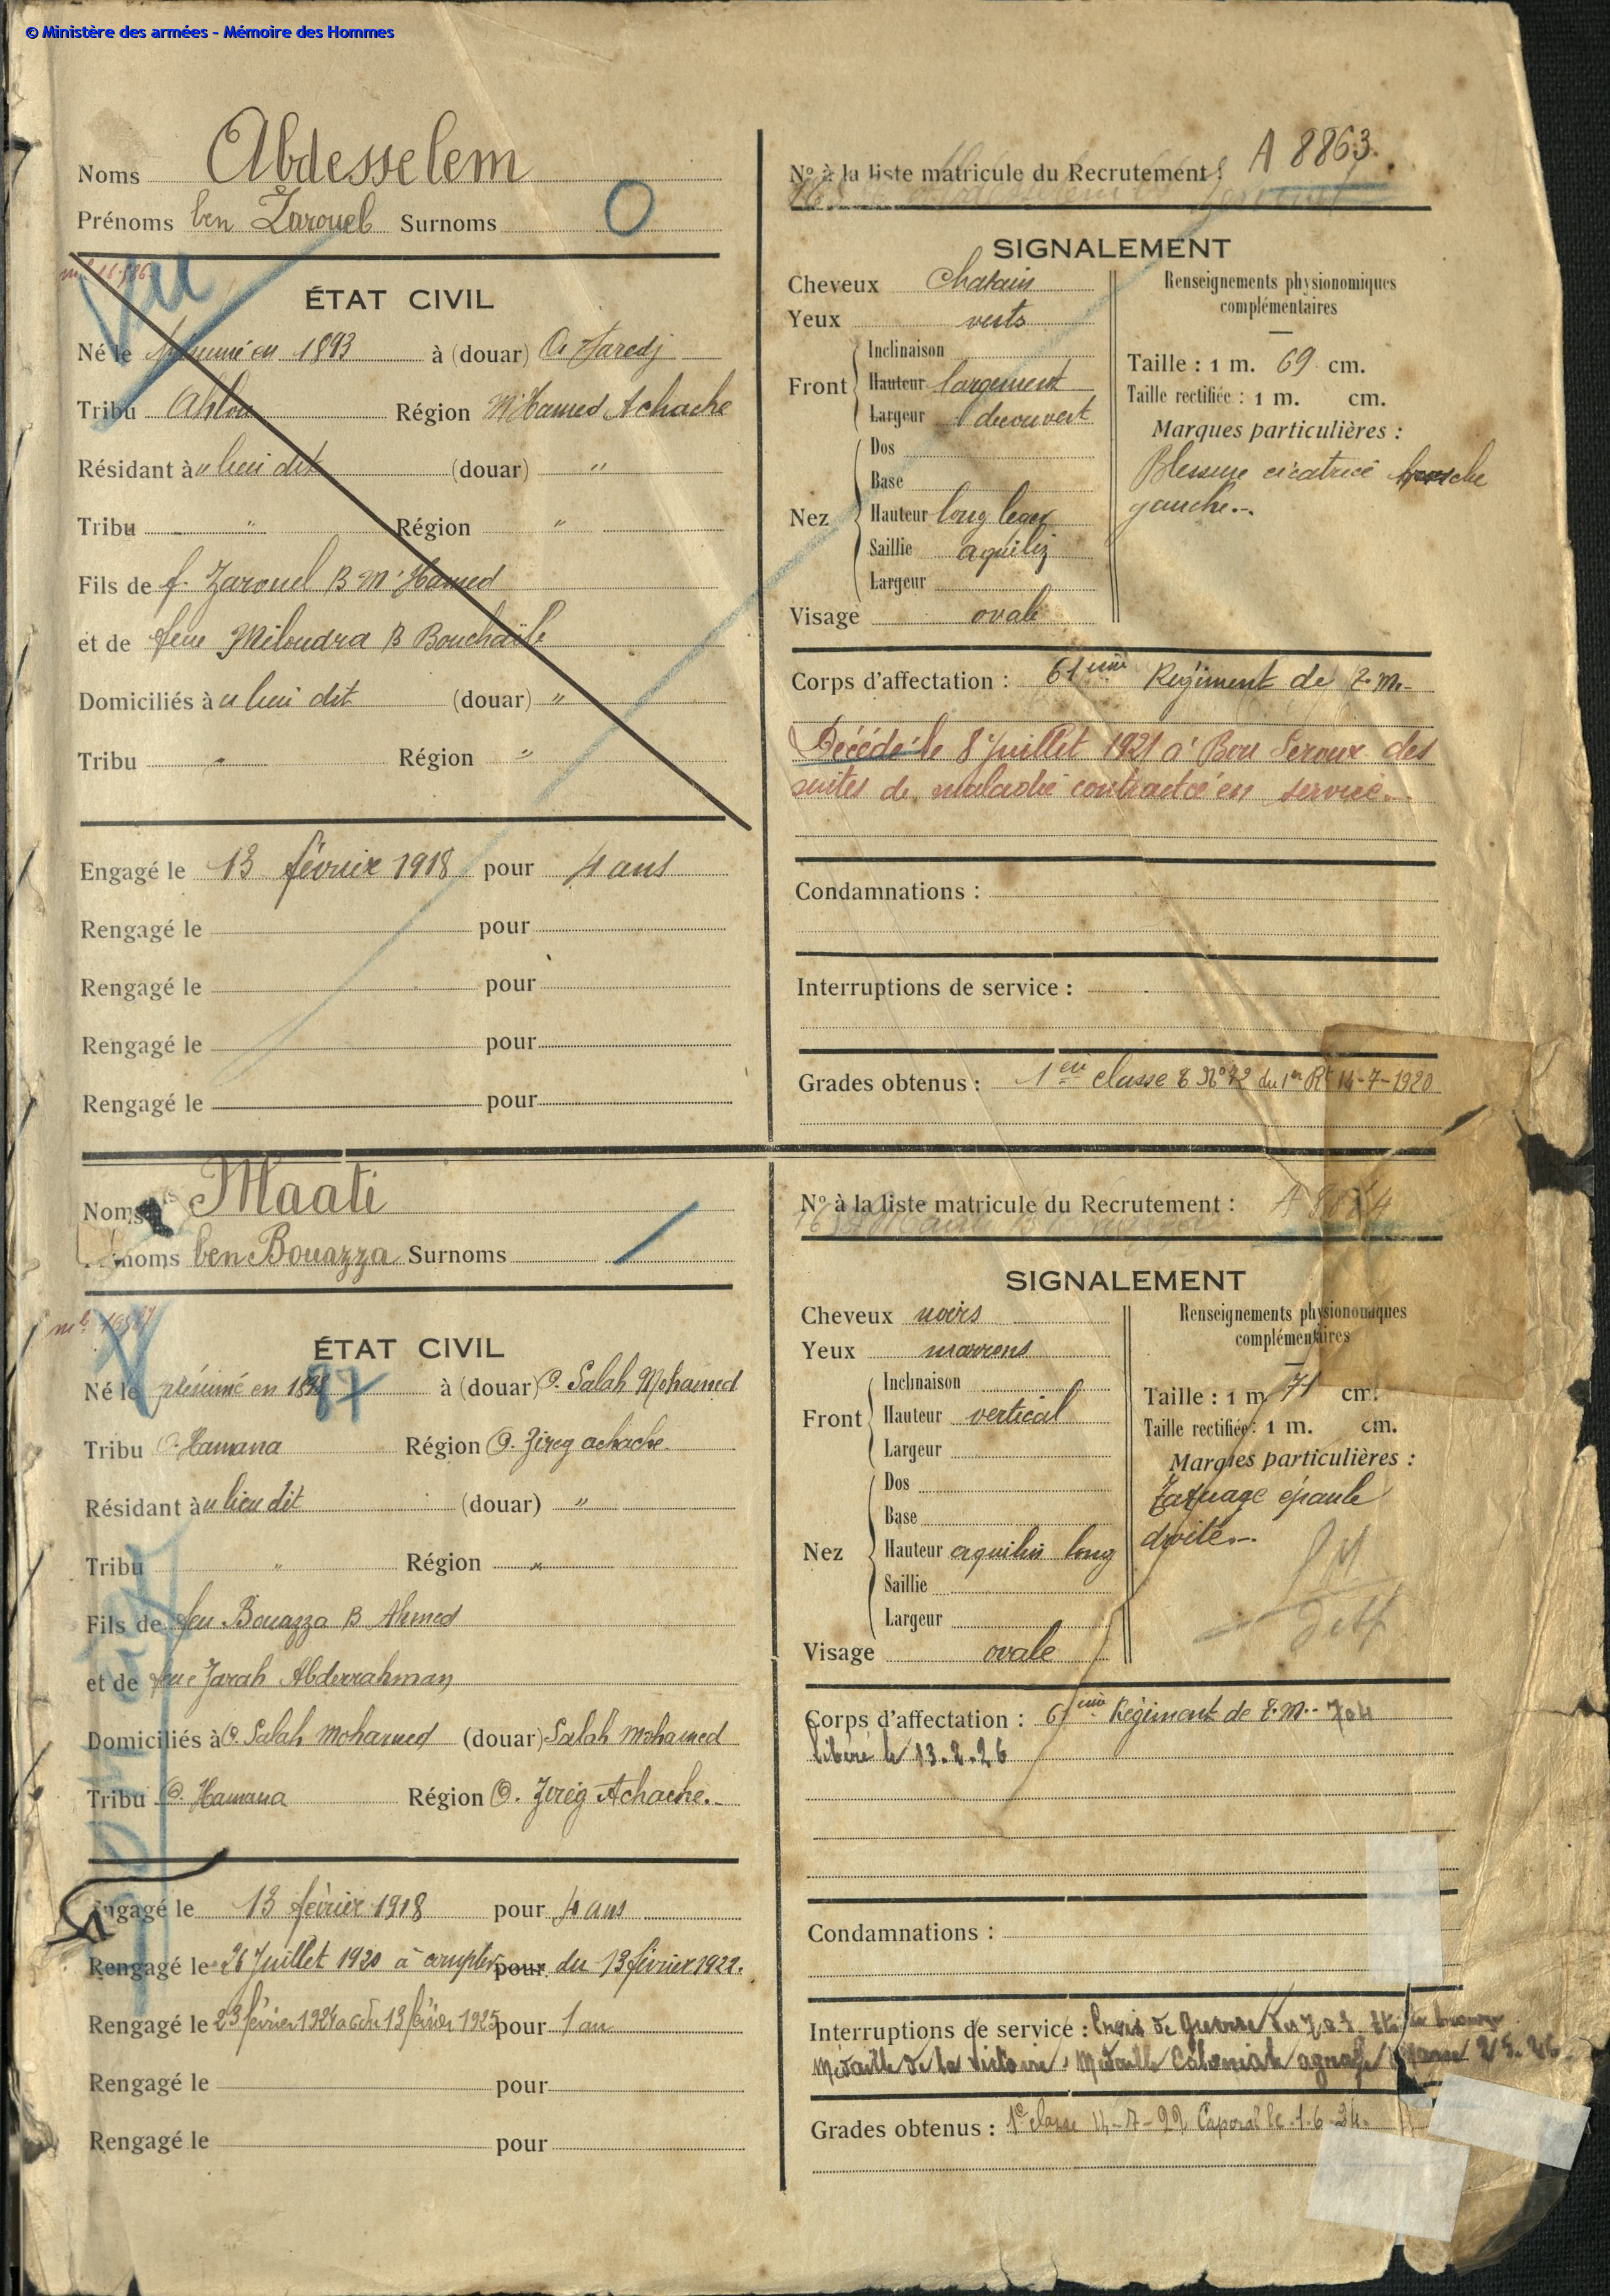
\includegraphics[scale=0.57]{Images/exemplemat2.jpeg}
        \caption[Note d'image]{Un exemple d'un registre matricule du Maroc\footnotemark}
    \label{fig:Mat 2}
    \end{center}
  \end{figure}
  \footnotetext{Source: \url{https://www.memoiredeshommes.sga.defense.gouv.fr/fr/article.php?larub=382&titre=recensement-des-engages-et-appeles-des-anciennes-colonies-francaises}
}

Comme vous pouvez le constater à travers les figures 1.2 et 1.3, les registre matricules sont des formulaires imprimés remplis avec des informations manuscrites. Même si les registres provenant des colonies tendent à être moins riches, ils contiennent le même type d’information que celles qui peuvent être  utiles dans le cadre d’une étude sur l’histoire militaire à grande échelle. On y trouve des indications telles que le corps d’affectation d’un soldat et un événement éventuel comme le décès d’un soldat ou le fait qu’il soit réformé. Elles sont indiquées par un trait noir qui barre l’état civil et l’intégralité de la fiche. Cette pratique est visible dans la figure 1.3 pour le soldat Abdesselem. \\

Étant donné que des unités combattantes de la Grande guerre (nord-africaine, coloniale et métropolitaine) ont également combattus dans  la guerre du Rif, il est possible qu’une quantité importante de registres soit déjà numérisée car ils font partie de la base des fiches matricules de la Grande guerre sur le site Mémoires des hommes. Pour vérifier cela, il serait intéressant de commencer une transcription. Toutes les  fiches matricules des soldats venant du Maroc et certaines d’Algérie sont conservées  au Centre des archives du personnel militaire (CAPM) à Pau. Alors que les fiches matricules des soldats métropolitains qui se trouvent sur les sites des différentes archives départementales sont organisées par classe et non pas par conflit, ce qui rend toute recherche impossible sans la transcription de ces fiches. Pour les soldats de l’armée coloniale (les troupes de marine) et l’armée d'Afrique en Algérie et Tunisie, certains des registres matricules sont numérisés jusqu’à la classe de 1921.\footnote{ Voir : \url{http://anom.archivesnationales.culture.gouv.fr/regmatmil/ 
}.} Le reste des ces registres se trouvent sous forme papier aux Archives nationales d’outre-mer (ANOM) à Aix-en-Provence.\\

\section{Les journaux des marches et opérations}
\urldef\myurl\url{https://www.memoiredeshommes.sga.defense.gouv.fr/fr/article.php%3Flarub%3D2%26titre%3Djournaux-des-unites-engagees-dans-la-premiere-guerre-mondiale}
Les journaux des marches et d'opérations sont les carnets de bord des grandes unités militaires, c'est-à-dire des unités de la taille d'un régiment ou plus. Ces journaux contiennent un large éventail d'informations, allant de la météo et des pertes subites jusqu’au moral des troupes à des moments précis. Il existe des exemples des ces journaux numérisés sur le site du SHD dans la base de données des journaux des unités ayant participées à la Grande Guerre, mais ceux des régiments de marche formés pendant la guerre du Rif, ni d’autres régiments ayant combattu dans cette guerre ne s’y sont pas.\footnote{Voir: \myurl.} Les journaux des marches et opérations (JMO) concernés par mon étude se trouvent actuellement au SHD de Vincennes dans la sous-série 3H des côtes 803 à 1175 qui contient les JMO de la campagne du Rif.\footcites[30]{shd2002} Les JMOs des goums, les unités supplétifs marocaines commandés par des officiers français qui permettraient d'éclairer une histoire encore plus méconnue que celles de troupes coloniales et nord-africaines se trouvent dans les côtes 2375 à 2711 de la même série.\footcites[33]{shd2002}\begin{figure}[h!]
    \begin{center}
      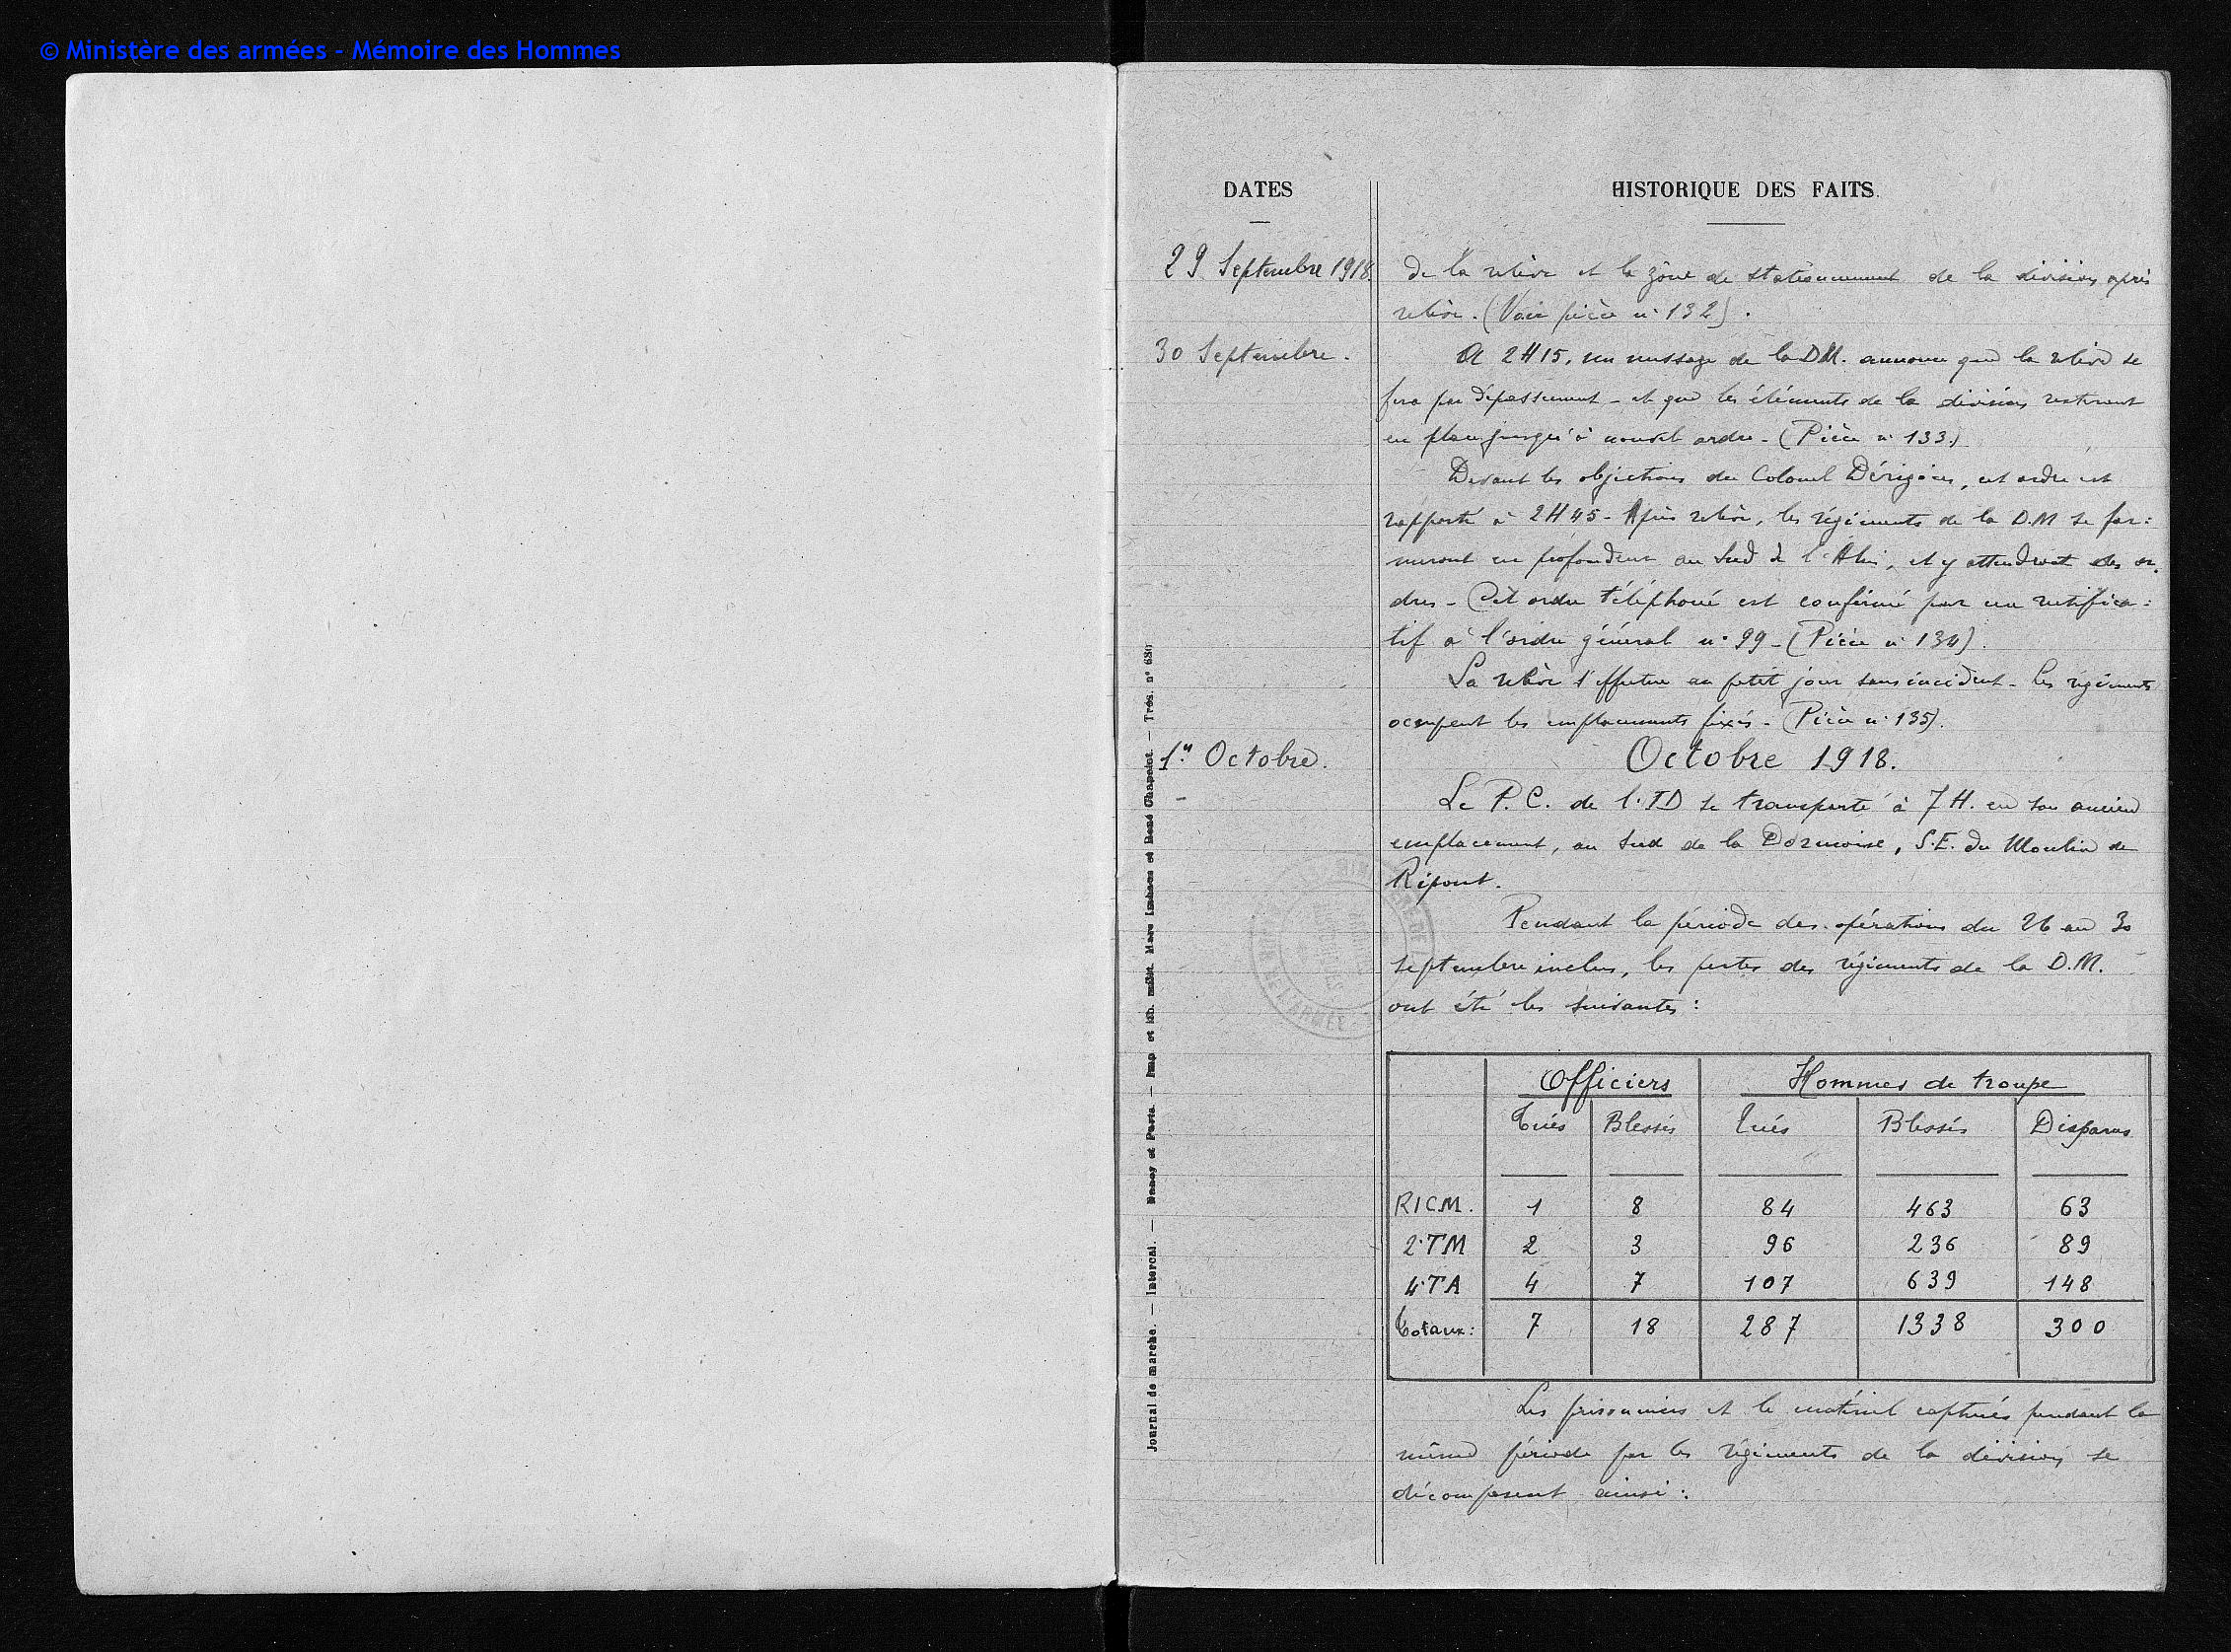
\includegraphics[scale=0.8]{Images/exemplejmo.jpeg}
        \caption[Note d'image]{Un exemple d'un journal des marches et d'opérations\footnotemark}
    \label{fig:JMO}
    \end{center}
  \end{figure}
  \footnotetext{Source: \myurl}

Comme le montre la figure 1.4, ces JMO peuvent constituer un contrôle extrêmement utile de la base de données fournie par le SHD ou de celle créée à partir des fiches matricules transcrites. En bas de page de l’image figure le nombre de pertes subies par la composante d’infanterie de la Division Marocaine  en 1918. Les différents régiments sont indiqués avec leurs pertes par types de soldat (les hommes de troupes et les officiers). En plus de fournir des informations sur les effectifs d’un régiment, les JMOs permettent de faire correspondre les pertes statistiques à des événements militaires tels qu’une offensive ou un siège.\\

\section{Conclusion}
La combinaison de ces trois sources différentes devrait donner un caractère particulier à cette étude. Ce qui ressort de leur utilisation combinée est leur nature équilibrante. En théorie, elles devraient agir comme des garde-fous pour toute conclusion globale que les résultats individuels pourraient suggérer. Couplé d’une lecture de la littérature secondaire et d’une analyse des archives qualitatives, le traitement de sources quantitatives devrait apporter de nouvelles perspectives sur l’histoire de cette guerre. 